% vim: tw=80

\chapter{Conclusion}

The proton PDFs enter into almost all cross section calculations at the LHC. Thus, a
profound knowledge of the PDFs is crucial for all precision measurements.
However, the high-$x$ region of the PDFs in particular is not yet well known and exhibits
large uncertainties.

This thesis presents a new dijet analysis, specifically developed to provide
constraints on the PDFs in the best possible way. For the first time,
triple-differential dijet cross sections are measured at the LHC.
Constraints on the PDFs are derived and the strong coupling constant is
determined.
\\[-6pt]
\begin{figure}[btp]
    \centering
    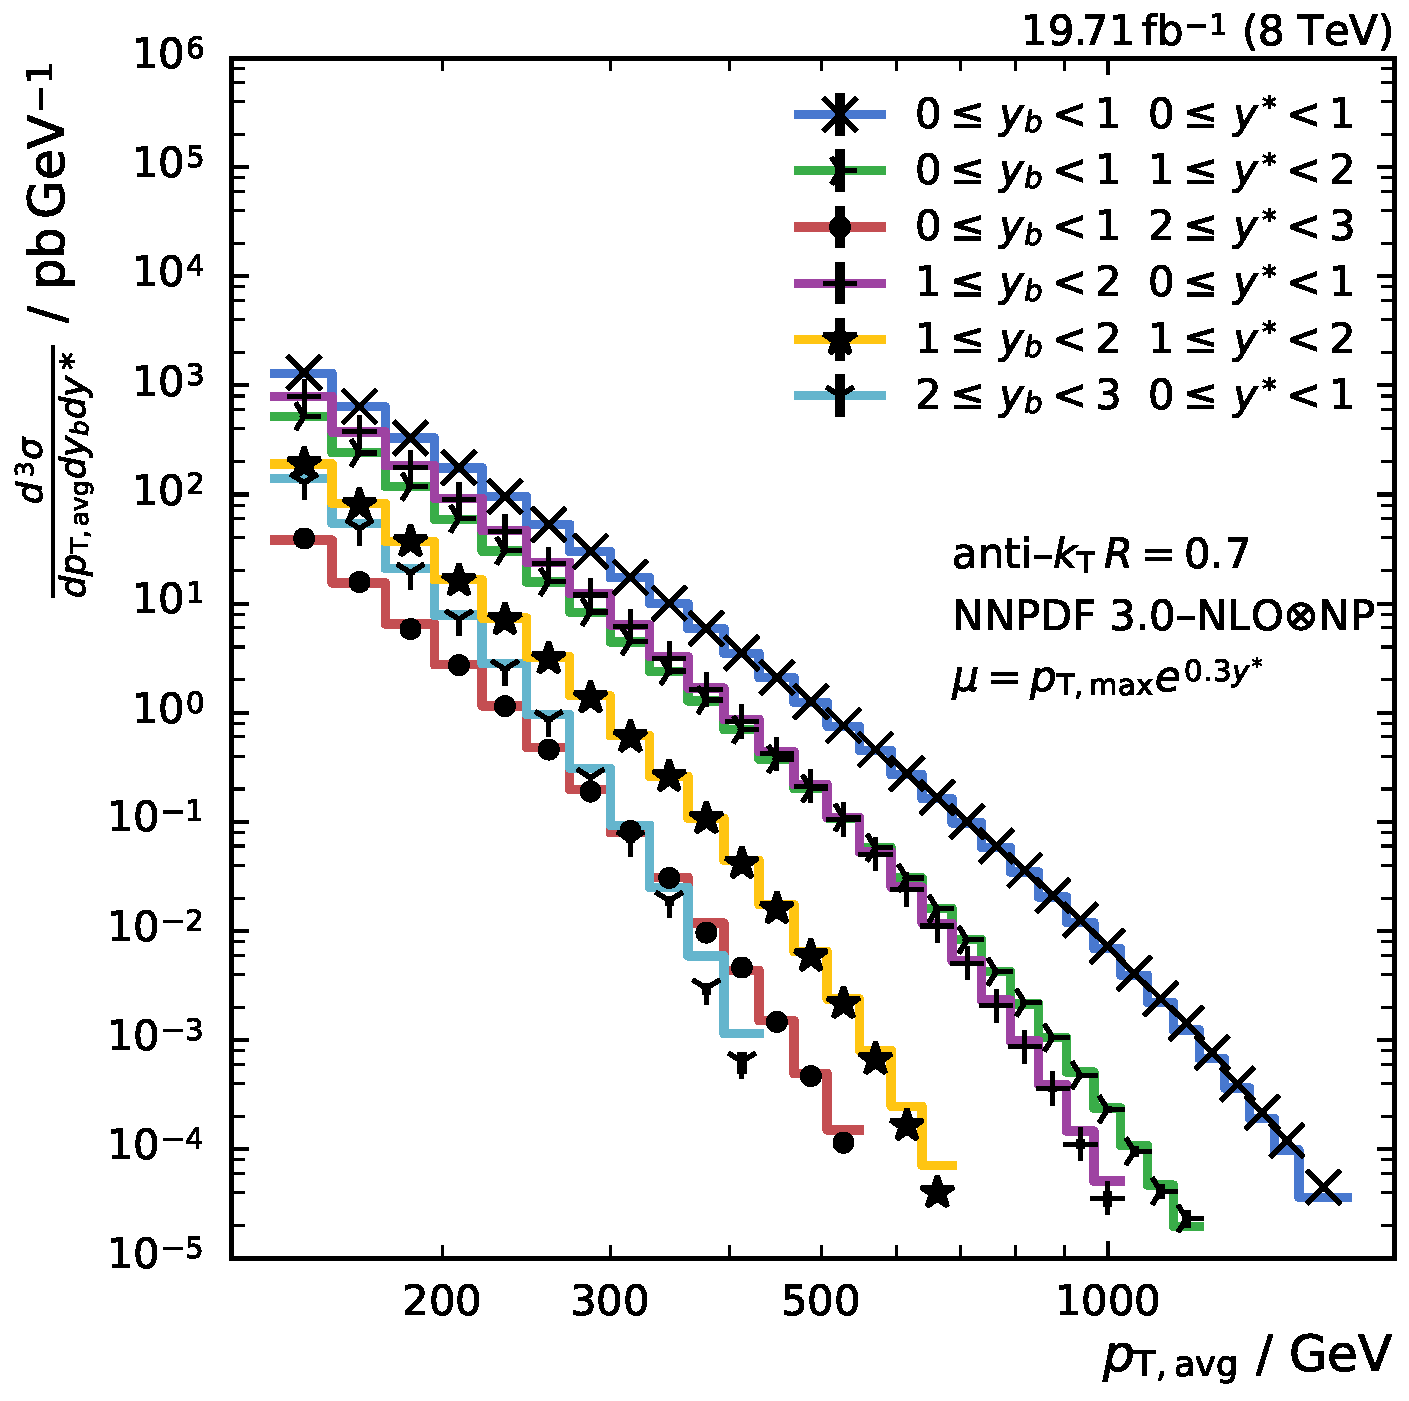
\includegraphics[width=0.47\textwidth]{figures/measurement/ptavg_spectrum.pdf}\hfill
    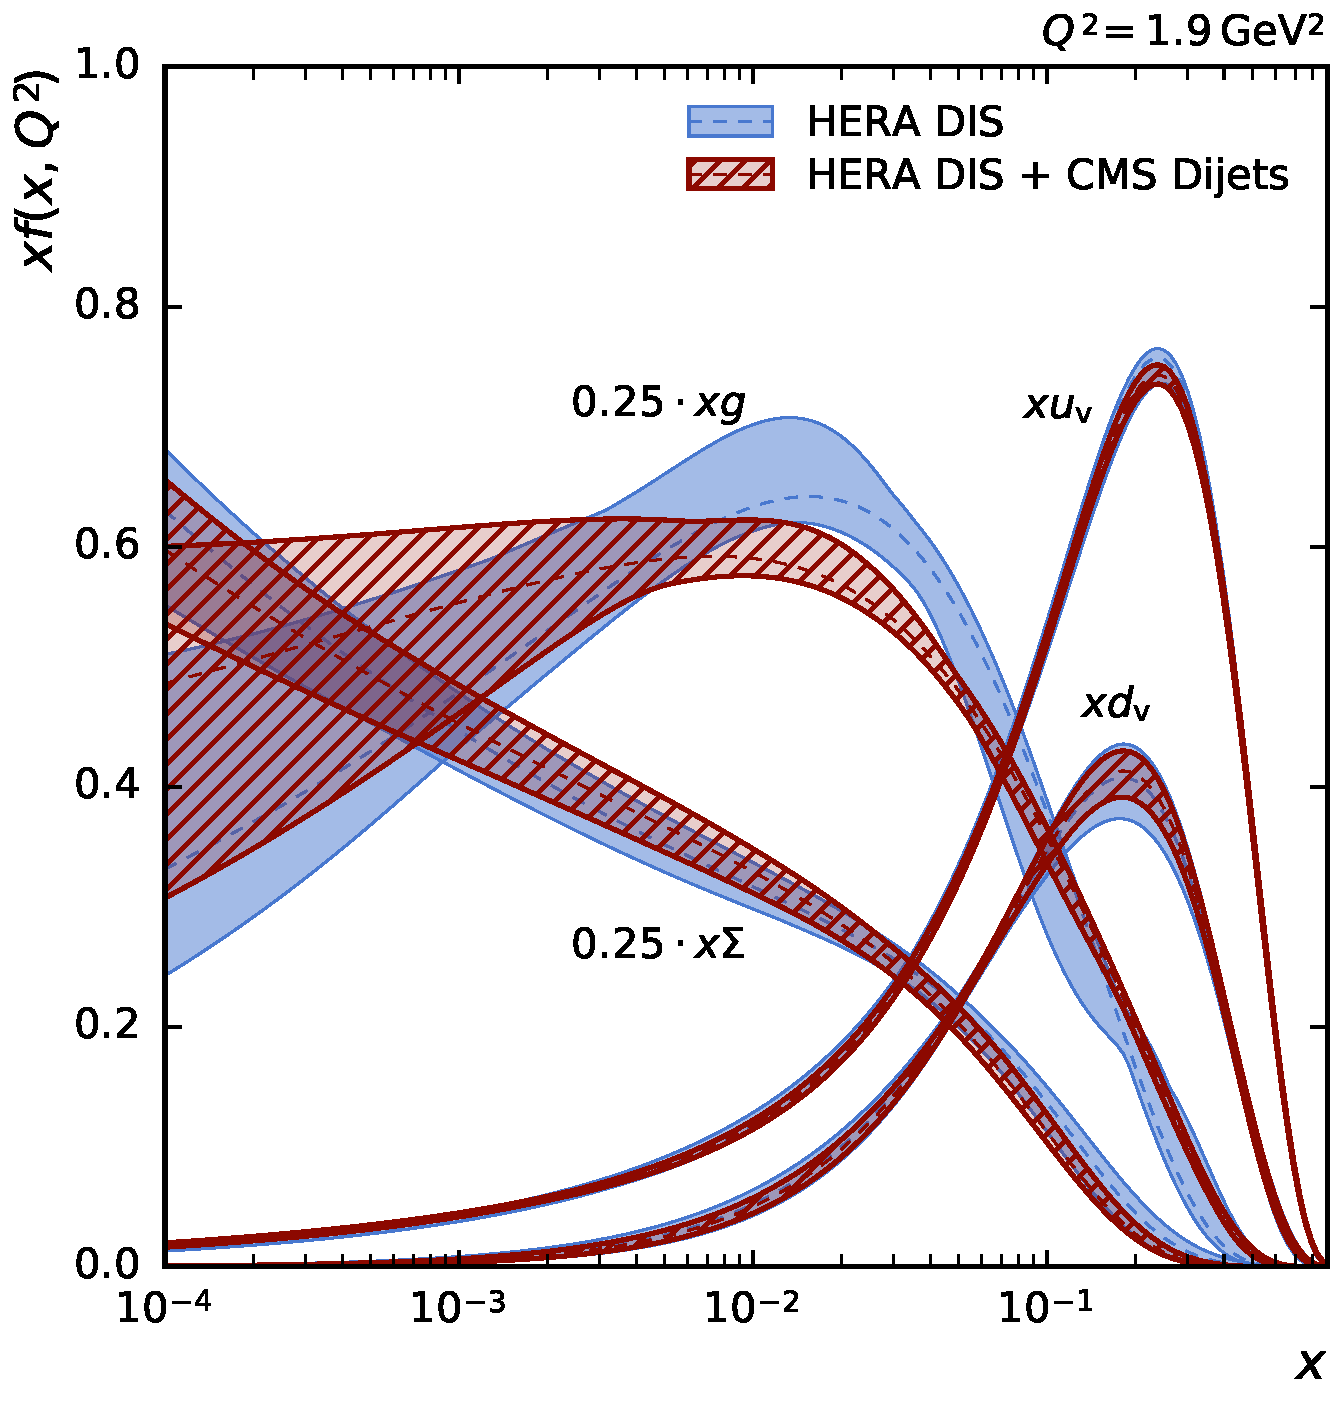
\includegraphics[width=0.45\textwidth]{figures/pdf_constraints/pdfcomp_direct_overview_1.9.pdf}
    \caption[Summary plot of results]{Left:
    The triple-differential dijet cross sections. The data are indicated by black
    markers, the NLO theory prediction by colored lines. Right: Overview of
    fitted PDFs with and without including the triple-differential dijet
    measurement.}
    \label{fig:conclusion}
\end{figure}

The measurement has been performed with the CMS detector at a center-of-mass
energy of \SI{8}{\TeV} using the complete data set recorded in 2012. The cross
sections are measured differentially as a function of the average transverse
momentum, the rapidity separation, and the boost of the dijet pair. Trigger,
reconstruction and detector effects were thoroughly studied. The measured cross
sections have been corrected for detector effects in an iterative unfolding
procedure. The unfolded cross sections are compared with pQCD predictions at NLO
accuracy which are corrected for non-perturbative effects. The data are well
described by the predictions over many orders of magnitude, see
Fig.~\ref{fig:conclusion}. In phase space regions with boosted dijet events, in
which the highest $x$ of the PDFs are probed, the predictions using different
global PDF sets exhibit large differences. The precise measurement discriminates
between them and constraints on the PDFs can thus be provided. 

The impact of the data on the PDFs is demonstrated by performing a PDF fit to
DIS cross sections obtained from the HERA experiments and the dijet cross sections measured
in this thesis. When the dijet data are considered, a harder gluon PDF is obtained
and the overall uncertainties of the PDFs are reduced. In particular the uncertainties of
the gluon PDF are drastically diminished in the high-$x$ region, see
Fig.~\ref{fig:conclusion} right.

The strong coupling constant \asmz has been determined together with the PDFs in
a simultaneous fit. The obtained value reads
%
\begin{equation*}
    \asmz = 0.1194_{-0.0015}^{+0.0015}\,(\mathrm{exp})\,
    {}_{-0.0002}^{+0.0002}\,(\mathrm{mod})\,{}_{-0.0004}^{+0.0002}\,(\mathrm{par})\,
    {}_{-0.0019}^{+0.0031}\,(\mathrm{scale})\,
\end{equation*}
%
and is in agreement with the world average value of $\asmz = 0.1181 \,\pm\, 0.0013$
determined by the PDG~\cite{Agashe:2014kda}. The dominant uncertainty is of
theoretical origin.

The pioneering studies presented in this thesis prove that the triple-differential
measurement of dijet cross sections using the chosen observables are an
excellent approach to perform QCD precision studies.

A few areas provide opportunities for further improvement: First, as NNLO
corrections for dijet calculations will become available in the near future, the
accuracy of the cross section predictions will be improved and the determination
of \asmz will profit from reduced scale uncertainties. Secondly, electroweak
corrections become relevant at transverse momenta beyond \SI{1}{\TeV}. By
considering them, the bins with highest \ptavg could be included in the fits as
well.

The restart of the LHC at an increased center-of-mass energy of $\SI{13}{\TeV}$,
coupled with a higher instantaneous luminosity, opens up a larger
accessible phase space. When CMS has collected a sufficiently large data sample,
it will be possible to extend this measurement to additional phase space regions
and improve the overall precision.

